% В этом файле следует писать текст работы, разбивая его на
% разделы (section), подразделы (subsection) и, если нужно,
% главы (chapter).

% Предварительно следует указать необходимую информацию
% в файле SETUP.tex

%% В этот файл не предполагается вносить изменения

% В этом файле следует указать информацию о себе
% и выполняемой работе.

\documentclass [fontsize=14pt, paper=a4, pagesize, DIV=calc]%
{scrartcl}
% ВНИМАНИЕ! Для использования глав поменять
% scrartcl на scrreprt

% Здесь ничего не менять
\usepackage [T2A] {fontenc}   % Кириллица в PDF файле
\usepackage [utf8] {inputenc} % Кодировка текста: utf-8
\usepackage [russian] {babel} % Переносы, лигатуры

%%%%%%%%%%%%%%%%%%%%%%%%%%%%%%%%%%%%%%%%%%%%%%%%%%%%%%%%%%%%%%%%%%%%%%%%
% Создание макроса управления элементами, специфичными
% для вида работы (курс., бак., маг.)
% Здесь ничего не менять:
\usepackage{ifthen}
\newcounter{worktype}
\newcommand{\typeOfWork}[1]
{
	\setcounter{worktype}{#1}
}

% ВНИМАНИЕ!
% Укажите тип работы: 0 - курсовая, 1 - бак., 2 - маг.,
% 3 - бакалаврская с главами.
\typeOfWork{1}
% Считается, что курсовая и бак. бьются на разделы (section) и
% подразделы (subsection), а маг. — на главы (chapter), разделы и
%  подразделы. Если хочется,
% чтобы бак. была с главами (например, если она большая),
% надо выбрать опцию 3.

% Если при выборе 2 или 3 вы забудете поменять класс
% документа на scrreprt (см. выше, в самом начале),
% то получите ошибку:
% ./aux/appearance.tex:52: Package scrbase Error: unknown option ` chapterprefix=

%%%%%%%%%%%%%%%%%%%%%%%%%%%%%%%%%%%%%%%%%%%%%%%%%%%%%%%%%%%%%%%%%%%%%%%%
% Информация об авторе и работе для титульной страницы

\usepackage {titling}

% Имя автора в именительном падеже (для маг.)
\newcommand {\me}{%
И.\,И.~Иванов%
}

% Имя автора в родительном падеже (для курсовой и бак.)
\newcommand {\byme}{%
Н.\,М.~Нежевского%
}

% Научный руководитель
\newcommand{\supervisor}%
{ст. преп. Брагилевский В.Н.}

% идентифицируем пол (только для курсовой и бак.)
\newcommand{\bystudent}{
Студента %Студентки % Для курсовой: с большой буквы
}

% Год публикации
\date{2016}

% Название работы
\title{Цветовая поддержка вывода консоли интерпретатора языка Haskell GHCi}

% Кафедра
%

\newcommand {\direction} {%
Направление подготовки\\02.\ifthenelse{\value{worktype} = 2}{04}{03}.02 ---
Фундаментальная информатика\\и информационные технологии%
}

%%%%%%%%%%%%%%%%%%%%%%%%%%%%%%%%%%%%%%%%%%%%%%%%%%%%%%%%%%%%%%%%%%%%%%%%
% Другие настраиваемые элементы текста

% Листинги с исходным кодом программ: укажите язык программирования
\usepackage{listings}
\lstset{
    language=[ISO]C++,%  Язык указать здесь
    basicstyle=\small\ttfamily,
    breaklines=true,%
    showstringspaces=false%
    inputencoding=utf8x%
}
% полный список языков, поддерживаемых данным пакетом, есть,
% например, здесь (стр. 13):
% ftp://ftp.tex.ac.uk/tex-archive/macros/latex/contrib/listings/listings.pdf

% Нумерация списков: можно при необходимести
% изменять вид нумерации (например, добавлять правую скобку).
% По умолчанию буду списки вида:
% 1.
% 2.
% Изменять вид нумерации можно в начале нумерации:
% \begin{enumerate}[1)] (В квадратных скобках указан желаемый вид)
\usepackage[shortlabels]{enumitem}
                    \setlist[enumerate, 1]{1.}

% Гиперссылки: настройте внешний вид ссылок
\usepackage%
[pdftex,unicode,pdfborder={0 0 0},draft=false,%backref=page,
    hidelinks, % убрать, если хочется видеть ссылки: это
               % удобно в PDF файле, но не должно появиться на печати
    bookmarks=true,bookmarksnumbered=false,bookmarksopen=false]%
{hyperref}


\usepackage {amsmath}      % Больше математики
\usepackage {amssymb}
\usepackage {textcase}     % Преобразование к верхнему регистру
\usepackage {indentfirst}  % Красная строка первого абзаца в разделе

\usepackage {fancyvrb}     % Листинги: определяем своё окружение Verb
\DefineVerbatimEnvironment% с уменьшенным шрифтом
	{Verb}{Verbatim}
	{fontsize=\small}

% Вставка рисунков
\usepackage {graphicx}

% Общее оформление
% ----------------------------------------------------------------
% Настройка внешнего вида

%%% Шрифты

% если закомментировать всё — консервативная гарнитура Computer Modern
\usepackage{paratype} % профессиональные свободные шрифты
%\usepackage {droid}  % неплохие свободные шрифты от Google
%\usepackage{mathptmx}
%\usepackage {mmasym}
%\usepackage {psfonts}
%\usepackage{lmodern}
%var1: lh additions for bold concrete fonts
%\usepackage{lh-t2axccr}
%var2: the package below could be covered with fd-files
%\usepackage{lh-t2accr}
%\usepackage {pscyr}

% Геометрия текста

\usepackage{setspace}       % Межстрочный интервал
\onehalfspacing

\newlength\MyIndent
\setlength\MyIndent{1.25cm}
\setlength{\parindent}{\MyIndent} % Абзацный отступ
\frenchspacing            % Отключение лишних отступов после точек
\KOMAoptions{%
    DIV=calc,         % Пересчёт геометрии
    numbers=endperiod % точки после номеров разделов
}

                            % Консервативный вариант:
%\usepackage                % ручное задание геометрии
%[%                         % (не рекомендуется в проф. типографии)
%  margin = 2.5cm,
  %includefoot,
  %footskip = 1cm
%] %
%  {geometry}

%%% Заголовки

\ifthenelse{\equal{\theworktype}{2}}{%
\KOMAoptions{%
    numbers=endperiod,% точки после номеров разделов
    headings=normal,   % размеры заголовков поменьше стандартных
    chapterprefix=true,% Печатать слово Глава в магистерской
    appendixprefix=true% Печатать слово Приложение
}
}

% шрифт для оформления глав и названия содержания
\newcommand{\SuperFont}{\Large\sffamily\bfseries}

% Заголовок главы
\ifthenelse{\value{worktype} > 1}{%
\renewcommand{\SuperFont}{\Large\normalfont\sffamily}
\newcommand{\CentSuperFont}{\centering\SuperFont}
\usepackage{fncychap}
\ChNameVar{\SuperFont}
\ChNumVar{\CentSuperFont}
\ChTitleVar{\CentSuperFont}
\ChNameUpperCase
\ChTitleUpperCase
}

% Заголовок (под)раздела с абзацного отступа
\addtokomafont{sectioning}{\hspace{\MyIndent}}

\renewcommand*{\captionformat}{~---~}
\renewcommand*{\figureformat}{Рисунок~\thefigure}

% Плавающие листинги
\usepackage{float}
\floatstyle{ruled}
\floatname{ListingEnv}{Листинг}
\newfloat{ListingEnv}{htbp}{lol}[section]

% точка после номера листинга
\makeatletter
\renewcommand\floatc@ruled[2]{{\@fs@cfont #1.} #2\par}
\makeatother


%%% Оглавление
\usepackage{tocloft}

% шрифт и положение заголовка
\ifthenelse{\value{worktype} > 1}{%
\renewcommand{\cfttoctitlefont}{\hfil\SuperFont\MakeUppercase}
}{
\renewcommand{\cfttoctitlefont}{\hfil\SuperFont}
}

% слово Глава
\usepackage{calc}
\ifthenelse{\value{worktype} > 1}{%
\renewcommand{\cftchappresnum}{Глава }
\addtolength{\cftchapnumwidth}{\widthof{Глава }}
}

% Очищаем оформление названий старших элементов в оглавлении
\ifthenelse{\value{worktype} > 1}{%
\renewcommand{\cftchapfont}{}
\renewcommand{\cftchappagefont}{}
}{
\renewcommand{\cftsecfont}{}
\renewcommand{\cftsecpagefont}{}
}

% Точки после верхних элементов оглавления
\renewcommand{\cftsecdotsep}{\cftdotsep}
%\newcommand{\cftchapdotsep}{\cftdotsep}

\ifthenelse{\value{worktype} > 1}{%
    \renewcommand{\cftchapaftersnum}{.}
}{}
\renewcommand{\cftsecaftersnum}{.}
\renewcommand{\cftsubsecaftersnum}{.}
\renewcommand{\cftsubsubsecaftersnum}{.}

%%% Списки (enumitem)

\usepackage {enumitem}      % Списки с настройкой отступов
\setlist %
{ %
  leftmargin = \parindent, itemsep=.5ex, topsep=.4ex
} %

% По ГОСТу нумерация должны быть буквами: а, б...
%\makeatletter
%    \AddEnumerateCounter{\asbuk}{\@asbuk}{м)}
%\makeatother
%\renewcommand{\labelenumi}{\asbuk{enumi})}
%\renewcommand{\labelenumii}{\arabic{enumii})}

%%% Таблицы: выбрать более подходящие

\usepackage{booktabs} % считаются наиболее профессионально выполненными
%\usepackage{ltablex}
%\newcolumntype {L} {>{---}l}

%%% Библиография

\usepackage{csquotes}        % Оформление списка литературы
\usepackage[
  backend=biber,
  hyperref=auto,
  sorting=none, % сортировка в порядке встречаемости ссылок
  language=auto,
  citestyle=gost-numeric,
  bibstyle=gost-numeric
]{biblatex}
\addbibresource{biblio.bib} % Файл с лит.источниками

% Настройка величины отступа в списке
\ifthenelse{\value{worktype} < 2}{%
\defbibenvironment{bibliography}
  {\list
     {\printtext[labelnumberwidth]{%
    \printfield{prefixnumber}%
    \printfield{labelnumber}}}
     {\setlength{\labelwidth}{\labelnumberwidth}%
      \setlength{\leftmargin}{\labelwidth}%
      \setlength{\labelsep}{\dimexpr\MyIndent-\labelwidth\relax}% <----- default is \biblabelsep
      \addtolength{\leftmargin}{\labelsep}%
      \setlength{\itemsep}{\bibitemsep}%
      \setlength{\parsep}{\bibparsep}}%
      \renewcommand*{\makelabel}[1]{\hss##1}}
  {\endlist}
  {\item}
}{}

% ----------------------------------------------------------------
% Настройка переносов и разрывов страниц

\binoppenalty = 10000      % Запрет переносов строк в формулах
\relpenalty = 10000        %

\sloppy                    % Не выходить за границы бокса
%\tolerance = 400          % или более точно
\clubpenalty = 10000       % Запрет разрывов страниц после первой
\widowpenalty = 10000      % и перед предпоследней строкой абзаца

% ----------------------------


% Стили для окружений типа Определение, Теорема...
% Оформление теорем (ntheorem)

\usepackage [thmmarks, amsmath] {ntheorem}
\theorempreskipamount 0.6cm

\theoremstyle {plain} %
\theoremheaderfont {\normalfont \bfseries} %
\theorembodyfont {\slshape} %
\theoremsymbol {\ensuremath {_\Box}} %
\theoremseparator {:} %
\newtheorem {mystatement} {Утверждение} [section] %
\newtheorem {mylemma} {Лемма} [section] %
\newtheorem {mycorollary} {Следствие} [section] %

\theoremstyle {nonumberplain} %
\theoremseparator {.} %
\theoremsymbol {\ensuremath {_\diamondsuit}} %
\newtheorem {mydefinition} {Определение} %

\theoremstyle {plain} %
\theoremheaderfont {\normalfont \bfseries} 
\theorembodyfont {\normalfont} 
%\theoremsymbol {\ensuremath {_\Box}} %
\theoremseparator {.} %
\newtheorem {mytask} {Задача} [section]%
\renewcommand{\themytask}{\arabic{mytask}}

\theoremheaderfont {\scshape} %
\theorembodyfont {\upshape} %
\theoremstyle {nonumberplain} %
\theoremseparator {} %
\theoremsymbol {\rule {1ex} {1ex}} %
\newtheorem {myproof} {Доказательство} %

\theorembodyfont {\upshape} %
%\theoremindent 0.5cm
\theoremstyle {nonumberbreak} \theoremseparator {\\} %
\theoremsymbol {\ensuremath {\ast}} %
\newtheorem {myexample} {Пример} %
\newtheorem {myexamples} {Примеры} %

\theoremheaderfont {\itshape} %
\theorembodyfont {\upshape} %
\theoremstyle {nonumberplain} %
\theoremseparator {:} %
\theoremsymbol {\ensuremath {_\triangle}} %
\newtheorem {myremark} {Замечание} %
\theoremstyle {nonumberbreak} %
\newtheorem {myremarks} {Замечания} %


% Титульный лист
% Макросы настройки титульной страницы
% В этот файл не предполагается вносить изменения

%\usepackage {showframe}

% Вертикальные отступы на титульной странице
\newcommand{\vgap}{\vspace{16pt}}

% Помещение города и даты в нижний колонтитул
\usepackage{scrlayer}
\DeclareNewLayer[
  foot,
  foreground,
  contents={%
    \raisebox{\dp\strutbox}[\layerheight][0pt]{%
      \parbox[b]{\layerwidth}{\centering Ростов-на-Дону\\ \thedate%
       \\\mbox{}
       }}%
  }
]{titlepage.foot.fg}
\DeclareNewPageStyleByLayers{titlepage}{titlepage.foot.fg}


\AtBeginDocument %
{ %
  %
  \begin{titlepage}
  %
    \thispagestyle{titlepage}

    {\centering
    %
    \MakeTextUppercase {МИНИСТЕРСТВО ОБРАЗОВАНИЯ И НАУКИ РФ}

    \vgap

    Федеральное государственное автономное образовательное\\
    учреждение высшего образования\\
    \MakeTextUppercase {Южный федеральный университет}

    \vgap

	Институт математики, механики и компьютерных наук
    имени~И.\,И.\,Воровича

    \vgap

    \direction

    \vspace* {\fill}

    \ifthenelse{\value{worktype} = 2}{%
    \me

    \vgap}{}

    {\usefont{T2A}{PTSansCaption-TLF}{m}{n}
    \MakeTextUppercase{\thetitle}}

    \ifthenelse{\value{worktype} = 2}{%
     \vgap

    Магистерская диссертация}{}
    \ifthenelse{\value{worktype} = 0}{
     \vgap

    Курсовая работа
    }{}%
    \ifthenelse{\value{worktype} = 1 \OR \value{worktype} = 3}{
     \vgap

    Выпускная квалификационная работа\\
    на степень бакалавра
    }{}%

    \vspace {\fill}

    \begin{flushright}
    \ifthenelse{\value{worktype} = 0 \OR 
                \value{worktype} = 1 \OR
                \value{worktype} = 3}{
      \bystudent \ifthenelse{\value{worktype} = 0}{3}{4}\ курса\\
      \byme
    }{}

    \vgap

    Научный руководитель:\\
    \supervisor\\
    \ifthenelse{\value{worktype} = 2}{%
    Рецензент:\\
    ученая степень, ученое звание, должность
    И. О. Фамилия
    }{}
	\end{flushright}
\ifthenelse{\value{worktype} = 0}{
\vspace{\fill}
        \begin{flushleft}
          \begin{tabular}{cc}
            \underline{\hspace{4cm}}&\underline{\hspace{5cm}}\\
            {\small оценка (рейтинг)} & {\small  подпись руководителя}\\
          \end{tabular}
          \\[1cm]
        \end{flushleft}
}{}
\ifthenelse{\value{worktype} = 1 \OR \value{worktype} = 3}{
\vspace{\fill}
        \begin{flushleft}
Допущено к защите:\\руководитель направления ФИИТ
\underline{\hspace{4cm}}
В.\,С.\,Пилиди
        \end{flushleft}
}{}


  	\vspace {\fill}
  %Ростов-на-Дону

    %\thedate
  }\end{titlepage}
  %
  %

  %
  \clearpage
} %


% Команды для использования в тексте работы


% макросы для начала введения и заключения
\newcommand{\Intro}{\addsec{Введение}}
\ifthenelse{\value{worktype} > 1}{%
    \renewcommand{\Intro}{\addchap{Введение}}%
}

\newcommand{\Conc}{\addsec{Заключение}}
\ifthenelse{\value{worktype} > 1}{%
    \renewcommand{\Conc}{\addchap{Заключение}}%
}

% Правильные значки для нестрогих неравенств и пустого множества
\renewcommand {\le} {\leqslant}
\renewcommand {\ge} {\geqslant}
\renewcommand {\emptyset} {\varnothing}

% N ажурное: натуральные числа
\newcommand {\N} {\ensuremath{\mathbb N}}

% значок С++ — используйте команду \cpp
\newcommand{\cpp}{%
C\nolinebreak\hspace{-.05em}%
\raisebox{.2ex}{+}\nolinebreak\hspace{-.10em}%
\raisebox{.2ex}{+}%
}

% Неразрывный дефис, который допускает перенос внутри слов,
% типа жёлто-синий: нужно писать жёлто"/синий.
\makeatletter
    \defineshorthand[russian]{"/}{\mbox{-}\bbl@allowhyphens}
\makeatother


\endinput

% Конец файла



\NewBibliographyString{langjapanese}
\NewBibliographyString{fromjapanese}

\begin{document}

\addsec{Постановка задачи}
\begin{enumerate}
  \item Анализ возможных подходов к реализации подсветки вывода
  \item Изучение программной структуры GHCi
  \item Программная реализация цветовой поддержки вывода интерпретатора GHCi
\end{enumerate}  

\newpage
  
\tableofcontents

\newpage

\Intro

GHC - один из наиболее развитых на сегодняшний день компиляторов функционального языка Haskell. В состав компилятора входит интерпретирующая интерактивная среда GHCi. GHCi используется для отображения результатов вызовов функций, отладочной информации, вывода типов и сортов функций.

Во многих интерактивных средах разработки поддерживается цветовое выделение  ключевых слов, констант и выражений в программном выводе. Такая возможность широко используется для обеспечения наглядности и удобности чтения и анализа программного вывода.

В настоящее время в состав GHC не входит встроенных средств для цветовой поддержки выводимого текста. Существуют программы, позволяющие частично решить данную задачу. В данной работе рассматривается программная реализация, обеспечивающая цветовую поддержку консольного вывода в интерпретаторе, а также анализируется программная составляющая GHC с точки зрения решения задачи цветовой поддержки вывода текстового результата в консоль.

\section{Решение на основе внешней обработки вывода}
\subsection{Алгоритм решения}
Одним из возможных решений является внешняя обработка выводимого интерпретатором GHCi текстового результата. Этот вариант удобен тем, что для его реализации нет необходимости изменять исходный код интерпретатора.

Обработка вывода интерпретатора GHCi должна работать по данному алгоритму:
\begin{enumerate}
  \item Внешняя программа-обработчик принимает пользовательский ввод;
  \item Этот пользовательский ввод передаётся в интерпретатор GHCi;
  \item Программа-обработчик перехватывает вывод результата GHCi;
  \item Этот результат обрабатывается и возвращается пользователю.
\end{enumerate}

Основной проблемой данного алгоритма является передача команд интерпретатору для обработки. GHC не предоставляет функционала для выполнения команд, подаваемых из внешней программы. Существует возможность построчного выполнения команд путём запуска компилятора GHC в интерактивном режиме со строкой-командой в параметре, однако в случае такого подхода теряется контекст выполнения, такой как значения вычисленных переменных.

\subsection{Программная реализация}
В рамках решения задачи цветовой поддержки вывода, была создана программная реализация, поддерживающая указанный алгоритм. Эта реализация является обёрткой над GHCi. Она представляет пользователю возможность консольного ввода команд, после чего эти команды передаются интерпретатору для вычисления. Результат вычислений обрабатывается во внешней программе, после чего выводится в консоль.

Проблема передачи выражений для вычисления компилятором GHC была решена использованием библиотеки ghcid. Данная библиотека позволяет запустить и использовать установленный в системе интерпретатор GHCi в фоновом режиме с полной поддержкой всего функционала. Для обращения к нему она предоставляет собственный API [1].

\newpage

\begin{lstlisting}[language=Haskell, caption=Пример выполнения входной строки с помощью ghcid]
(ghci, _) <- startGhci "ghci" (Just ".") True
let executeStatement = exec ghci
input <- getLine
result <- executeStatement input
\end{lstlisting}

В этом примере вводимая команда содержится в переменной input. Функция executeStatement передаёт введённую команду запущенному в фоне ghci и возвращает результат. Результат возвращается как набор строк в монаде IO и извлекается в переменную result.

После получения результатов из GHCi, набор строк передаётся парсеру. Парсер выделяет из строки элементы, которым необходимо добавить окраску. К данным элементам он добавляет информацию о типе подстроки. Информация о типе используется в дальнейшем для выбора параметров окраски.

\begin{lstlisting}[language=Haskell]
data SDoc next =
  SEmpty
  | SText String (SDoc next)
  | SToken Token (SDoc next)
\end{lstlisting}

SToken содержит некоторое выражение, которое необходимо окрасить и дополнительную информацию о типе выражения. Этот тип используется в дальнейшем для окраски выделенной подстроки. Если же подстрока не распознаётся, то она заносится в SText, и в дальнейшем никак дополнительно не обрабатывается.

\begin{lstlisting}[language=Haskell]
data Token =
  Arrow            String
  | Bracket        String
  | Digit          String
  | Typeclass      String
  | Type           String
  | CompileInfo    String 
  | Keyword	   String
\end{lstlisting}

В листинге представлена функция-парсер, генерирующая из строки выражение типа SDoc.

\begin{lstlisting}[language=Haskell, caption = Функция парсинга выражения]
parseExpression :: String -> SDoc next
parseExpression "" = SEmpty
parseExpression str
  | isStartsWithArrow str
    = SToken (Arrow (extractArrow str)) (parseExpression . dropArrow $ str)
  | isStartsWithBracket str
    = SToken (Bracket (extractBracket str)) (parseExpression . dropBracket $ str)
  | isStartsWithTypeclass str
    = SToken (Typeclass (extractTypeclass str)) (parseExpression . dropTypeclass $ str)
  | isStartsWithType str
    = SToken (Type (extractType str)) (parseExpression . dropType $ str)
  | isStartsWithInfo str
    = SToken (CompileInfo (extractCInfo str)) (parseExpression . dropCInfo $ str)
  | isStartsWithKeyword str
    = SToken (Keyword (extractKeyword str)) (parseExpression . dropKeyword $ str)
  | otherwise
    = SText (extractWord str ) (parseExpression . dropWord $ str)
\end{lstlisting}

После построения выражения типа SDoc, функция-визитор colorize осуществляет проход по нему. Подвыражения типа SToken окрашиваются и преобразуются в тип SText с удалением информации о содержащемся типе. Окрашивание происходит добавлением ANSI символов.

\begin{lstlisting}[language=Haskell, caption=Окрашивание выражения]
colorize :: SDoc next -> SDoc next
colorize SEmpty           = SEmpty
colorize (SToken token n) = SText (colorizeToken token) (colorize n)
colorize (SText str n)    = SText str (colorize n)
\end{lstlisting}

Функция colorizeToken используется для окраски выражения, содержащегося в подвыражении. Он использует информацию, представленную типом Token для выбора цвета окраски данной строки.

\begin{lstlisting}
colorizeToken :: Token -> String
colorizeToken (Arrow arrow) = clr SRed arrow
colorizeToken (Bracket bracket) = clr SBlue bracket
...
\end{lstlisting}

Список доступных цветов описан в типе-перечислении SColor.

\begin{lstlisting}[language=Haskell]
data SColor = 
   SRed
 | SBlue
 | SGreen
 | ...
\end{lstlisting}

Тип-перечисление SColor имеет реализацию класса типов Show. С его помощью можно получить строковое представление указанного цвета.

\begin{lstlisting}[language=Haskell]
instance Show SColor where
  show SRed    = "\x1b[31m"
  show SGreen  = "\x1b[32b"
  ...
\end{lstlisting}

Функция добавления ANSI символов clr получает строковое представление передаваемого цвета и имеет следующий вид.

\begin{lstlisting}[language=Haskell]
clr :: SColor -> String -> String
clr col str = (show col) ++ str ++ (show getDefaultColor)
\end{lstlisting}

После данных преобразований, исходное выражение типа SDoc содержит последовательность строк с имеющимся цветовым выделением. Функция concat' проходит по полученному выражения, преобразуя его в строку.

\begin{lstlisting}[language=Haskell]
concat' :: SDoc next -> String
concat' SEmpty = ""
concat' (SText subStr subSDoc) = subStr ++ (concat' subSDoc)
\end{lstlisting}

\newpage

На представленном ниже скриншоте продемонстрирован пример работы интерпретатора GHCi c использованием полученной реализации. При работе использовался GHC 7.8.4. На скриншоте показано цветовое выделение текстовых и численных констант, а также встроенных в GHC типов и классов типов.

\centerline{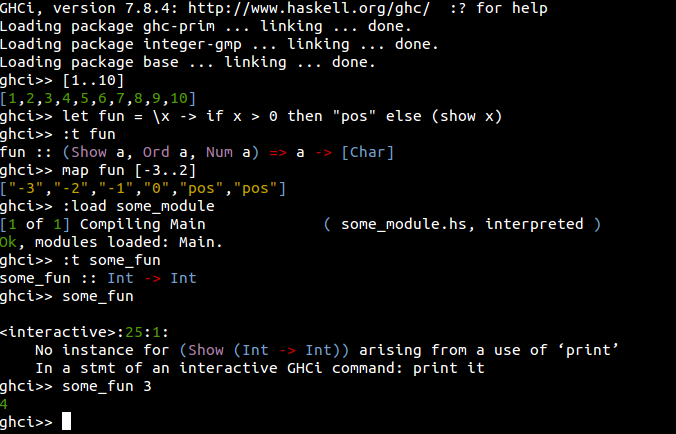
\includegraphics[scale=0.75]{img/example.png}}
\subsection{Сравнение реализаций}
В рамках сравнения реализаций, рассмотрим скрипт ghci-color, используемый для задачи окрашивания вывода [2].

Скрипт ghci-color также использует внешнюю обработку текстового вывода. Это достигается использованием потокового текстового редактора sed. Sed получает входной поток, преобразует каждую строку строку, согласно записанным в скрипт правилам, а затем выводит результат в выходной поток. Правила в скрипте основываются на регулярных выражениях. К подстроке, распознающейся регулярным выражением, добавляются ANSI символы.

Несмотря на схожий принцип действия, данные реализации имеют различия. Для использования ghci-color необходимо устанавливать текстовый редактор sed. Кроме того, в текущей реализации sed отсутствует подсветка типов и классов типов. Масштабирование скрипта с правилами затруднено тем, что для каждого нового элемента необходимо добавлять новое правило на основе регулярных выражений.

\subsection{Анализ полученных результатов}
Полученная реализация решает поставленную задачу по окраске вывода интерпретатора GHCi, однако обладает рядом недостатков:

\begin{enumerate}
\item Программа может обеспечить корректную окраску только для стандартных имён, так как не обладает информацией об определенных пользователем типах, классах типов и переменных
\item В некоторых ОС необходимы дополнительные действия по обеспечению корректной работы подсветки на основе ANSI символов
\item Со стороны пользователя требуются дополнительные действия для запуска данной программы, и её дальнейшего использования
\end{enumerate}

Таким образом, полученная программа решает поставленную задачу по окраске вывода GHCi. Однако, с учётом указанных выше недостатков, решение можно считать частичным.

\section{Система печати в GHCi}
Система печати в компиляторе GHC основана на принципе структурной печати. Принцип структурной печати заключается в том, что программа манипулирует абстрактными текстовыми элементами, комбинациями и операциями над ними. В результате манипуляций генерируется форматированный текст, чьё представление не зависит от конечной цели выводимого текста [3].

Основном примитивом в модели структурной печати является тип Doc, находящийся в модуле Pretty.
\begin{lstlisting}[language=Haskell]
data Doc
 = Empty
 | NilAbove Doc
 | Nest FastInt Doc
 | Union Doc Doc
 | ...
\end{lstlisting}

Тип Doc является абстракцией над своим содержимым. Тип Doc может представлять текстовые элементы, операции над текстовыми элементами или объединение других элементов типа Doc. Для типа Doc определено множество операций конкатенации, форматирования, выравнивания и вывода.

Тип SDoc является обёрткой над типом Doc. SDoc содержится в модуле Outputable. Тип SDoc содержит дополнительную информацию для обработки и печати содержащихся элементов в Doc.

\begin{lstlisting}[language=Haskell]
type SDoc = PprStyle -> Doc

data PprStyle
  = PprUser PrintUnqualified Depth
  | PprCode CodeStyle
  | PprDump
  | PprDebug
\end{lstlisting}

Тип-перечисление PprStyle содержит варианты вывода текста в Doc. Тип Doc и система печати может использоваться для пользовательского вывода, отладочного вывода или печати текста самой программы.

В языке Haskell класс типов содержит сигнатуры функций, применяемых к значениям некого типа. [4] Класс типов Outputable предоставляет интерфейс для типов, поддерживающих функцию структурной печати. Для большинства встроенных типов в Haskell имеется поддержка Outputable.

\begin{lstlisting}[language=Haskell]
class Outputable a where
	ppr :: a -> SDoc
\end{lstlisting}

Класс типов Outputable имеет одну функцию ppr, которая переводит выражение исходного типа в соответствующее ему выражение типа SDoc. Это выражение типа SDoc содержит текстовое представление исходного выражения, а также информацию о том, как необходимо выводить данный элемент. Например, функция ppr для типа Int имеет следующий вид:

\begin{lstlisting}[language=Haskell]
instance Outputable Int where
    ppr n = int n

int n = \ _ -> (text $ show n)

\end{lstlisting}

Для конечного преобразования элементов типа Doc в строки и их вывода, используется функция рендеринга текста, входящая в состав модуль Pretty.

\begin{lstlisting}[language=Haskell, caption=Типовая аннотация к функции рендеринга текста]
render :: Handle -> SDoc -> IO ()
\end{lstlisting}

Тип Handle необходим для операций чтения/записи с файлом или консолью. В данном случае он используется для вывода текста.

Текущая реализация класса типов Outputable и типа SDoc не поддерживает указание цвета данного элемента, поэтому для решения задачи по добавлению окраски вывода необходимо изменить их реализации.

\section{Необходимые изменения в модуле Outputable}

Работа с системой печати в GHC затруднена тем, что для существенных изменений в интерфейсе модуля печати, требуется изменение большого количества стороннего исходного кода. Поэтому была разработана модель структурная печати, аналогичная используемой в GHC. Данная модель поддерживает ограниченное количество типов и структурных операций, поэтому подходит для анализа и применения изменений. На основе этой модели были получен список изменений. Применение данных изменений в системе печати GHC позволит добавить встроенную цветовую поддержку.

\subsection{Изменения в модуле Outputable}

В текущей реализации тип SDoc содержит информацию только о формате вывода. Поэтому обёртка SDoc нуждается в расширении. Тип-перечисление PprStyle в SDoc необходимо заменить на тип SDocStyle, который будет содержать информацию о формате вывода и о цвете данного участка текста. Это позволит указывать, каким цветом необходимо выводить данный участок. Указание происходит в момент конструирования выражения типа SDoc.

\begin{lstlisting}[language=Haskell, caption=Дополненная реализация типа SDoc]
type SDoc = SDocStyle -> Doc
data SDocStyle = {
    pprStyle :: PprStyle,
    pprColor :: PprColor
}
type PprColor =
   CDefault
 | CRed
 | CBlue
 | ...
\end{lstlisting}

Примером работы с обёрткой при изменении цвета, является функция colorize. Ввиду неизменяемости данных в языке Haskell, функция colorize изменяет информацию о цвете путем создания нового элемента типа SDoc, содержащего новый цвет.

\begin{lstlisting}[language=Haskell, caption=Пример функции окраски]
colorize :: PprColor -> SDoc -> SDoc
colorize newPprColor sDoc = (newSDocStyle -> docContent)
  where 
    docContent = sDoc createEmptyStyle
    sDocStyle = pprStyle sDoc  
    newSDocStyle = SDocStyle { 
      pprStyle = pprStyle sDocStyle, 
      pprColor = newPprColor 
    }
\end{lstlisting}

Для поддержки цветового выделения всеми типами, необходим новый класс типов ColorOutputable. Чтобы поддерживать ColorOutputable, тип должен иметь поддержку Outputable. Для полной поддержки введённых изменений, необходимо полностью заменить Outputable на ColorOutputable во всех участках кода, где создаются элементы типа SDoc. Также ColorOutputable должен поддерживать все операции комбинирования, используемые в структурной печати.

\begin{lstlisting}[language=Haskell, caption=Класс типов ColorOutputable]
class Outputable a => ColorOutputable a where
  cppr :: a -> SDoc
\end{lstlisting}

Для получения соответствующего элемента типа SDoc на основании выражения исходного типа, функция cppr использует функцию ppr. После чего к выражению добавляется информация о цвете. Если данный элемент не требует окрашивания, то его значением цвета указывается CDefault. При дальнейшей генерации выводимого текста, этот элемент дополнительно не обрабатывается и выводится в стандартном цвете.

\begin{lstlisting}[language=Haskell, caption=Пример реализации ColorOutputable для типа Int]
instance ColorOutputable Int where
  cppr n = (colorize CBlue) . ppr $ n
\end{lstlisting}

Полученная информация о цвете используется при получении строкового представления из элементов типа SDoc. Функция colorizeDoc получает окрашенный вариант элемента типа Doc.

\begin{lstlisting}[language=Haskell]
colorizeDoc :: String -> String -> Doc -> Doc
colorizeDoc newColorStr defColorStr doc = (ptext newColorStr) <+> doc <+> (ptext defColorStr)
\end{lstlisting}

Операция (<+>) имеет указанную ниже сигнатуру и используется для конкатенации элементов типа Doc.
\begin{lstlisting}[language=Haskell]
(<+>) :: Doc -> Doc -> Doc
\end{lstlisting}

\subsection{Примеры с внедренными изменениями}
Для иллюстрации применения полученных изменений, рассмотрим модификации нескольких стандартных функций, аналоги которых были реализованы в модели.

Функция mkExpectedActualMsg, входящая в модуль TcErrors генерирует сообщение о несоответствии типов. Этот поддокумент состоит из ожидаемого типа и полученного типа.

\begin{lstlisting}[language=Haskell]
mkExpectedActualMsg :: Type -> Type -> SDoc
mkExpectedActualMsg exp_ty act_ty
  = vcat [ ptext (text "Expected type:") <+> ppr exp_ty
         , ptext (text "  Actual type:") <+> ppr act_ty ]
\end{lstlisting}

В функции mkExpectedActualMsg возможно добавить цветовое выделение для текстовых констант и передаваемых параметром типов. Тип Type имеет реализацию для Outputable, поэтому для него возможно реализовать класс типов ColorOutputable. В листинге цветовое выделение типа Type происходит с помощью функции cppr. Тип String не имеет реализации для Outputable, поэтому для него нельзя реализовать ColorOutputable. В данном примере окраска строковых констант выполняется вручную.

\begin{lstlisting}[language=Haskell, caption=Реализация функции с изменениями]
mkExpectedActualMsg :: Type -> Type -> SDoc
mkExpectedActualMsg exp_ty act_ty
  = vcat [ colorize cRed $ ptext (text "Expected type:") <+> cppr exp_ty
         , colorize cRed $ ptext (text "  Actual type:") <+> cppr act_ty ]
\end{lstlisting}

На приведённом скриншоте иллюстрируется полученное цветовое выделение.

\centerline{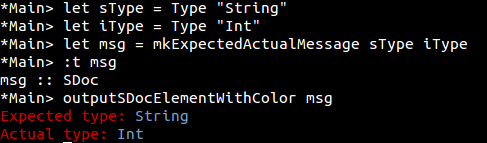
\includegraphics{img/example1.png}}

Функция srcParseErr входит в состав парсера компилятора GHC. Она генерирует сообщение о возникновении ошибки в пользовательском вводе в консоли интерпретатора GHCi. Ошибка возникает в случае ошибки при разборе входного выражения (например, это может быть забытая скобка). Текст данной функции представлен в листинге.

\begin{lstlisting}[language=Haskell]
srcParseErr :: ParserFlags -> StringBuffer -> Int -> SDoc
srcParseErr options buf len = if null token
         then ptext (text "parse error (possibly incorrect indentation or mismatched brackets)")
         else ptext (text "parse error on input" <+> quotes (text token))
  where token = ...    
\end{lstlisting}
\newpage
В данном примере добавляется цветовое выделение для строки-сообщения "parse error". Также добавляется выделение для неправильно введённого значения.

\begin{lstlisting}[language=Haskell]
srcParseErr :: ParserFlags -> StringBuffer -> Int -> SDoc
srcParseErr options buf len = if null token
         then parseErrorMsg <+> ptext (text "(possibly incorrect indentation or mismatched brackets)")
         else parseErrorMsg <+> ptext (text " on input" <+> quotes (colorize CBlue $ (text token))
  where 
    parseErrorMsg = colorize cRed $ ptext (text "parse error")
    token = ...    
\end{lstlisting}

На основании приведённых выше примеров модификации стандартных функций, можно сделать вывод, что внедрение полученных на основе модели изменений в систему печати GHCi будет достаточно, для обеспечения цветовой поддержки вывода консоли интерпретатора GHCi.


\Conc
В результате работы была создана программная реализация, решающая поставленную задачу по цветовой поддержки вывода консоли интерпретатора GHCi. Полученная реализация имеет ряд указанных ограничений.

Была проанализирована реализация вывода, используемая в GHC. На основе этой реализации была создана программная модель вывода, действующая аналогично системе вывода компилятора GHC. С помощью данной модели был получен список изменений, применение которых к  системе вывода GHC позволит реализовать встроенную цветовую поддержку.

\addsec{Список литературы}
\begin{enumerate}
  \item Библиотека ghcid. -- URL: https://github.com/ndmitchell/ghcid (дата обр. 05.05.2016)
  \item Скрипт ghci-color. -- URL: https://github.com/rhysd/ghci-color (дата обр. 06.05.2016)
  \item Документация по компилятору GHC -- URL: https://downloads.haskell.org/~ghc/7.10.2/docs/html/ (дата обр. 30.04.2016)
  \item Bryan O'Sullivan -- Real World Haskell. -- URL: http://book.realworldhaskell.org/ (дата обр 25.04.2016)
\end{enumerate}

\end{document}